\section{$^{24}$Mg}
In the following section, results for $^{24}$Mg are presented, it's a natural choice to study how well deformations are represented by our framework, since it's light, very deformed and shows no pairing interaction in its ground state.
\subsubsection{Ground state}
Table \ref{tab:mg_table} reports data for the ground state of $^{24}$Mg, while figure \ref{fig:mg_gs_density_axial} shows the total particle density.
\begin{table}[ht]
  \centering
  \begin{tabular}{lrrccc}
    \addlinespace[0.3em]
    \toprule
    && GCG & & $\Delta$ & $\Delta\%$ \\
    \midrule
    $E_{\text{TOT}}$& [MeV]    & -195.854 & & &  \\
    $\expval{ r^2_n}^{1/2}$    &[fm] & 3.0124    &  &  & \\
    $\expval{ r^2_p}^{1/2}$    &[fm] & 3.0475    &  &  & \\
    $\expval{ r^2_{ch}}^{1/2}$ &[fm] & 3.5390    &  &  & \\
    $\expval{z^2}^{1/2}$ &[fm] & 2.1454 &  &  &\\
    $\expval{x^2}^{1/2}$ &[fm] & 1.5112 &  &  &\\
    $\expval{y^2}^{1/2}$ &[fm] & 1.5147 &  &  &\\
    $\beta_2$ &[-] & 0.399 & & & \\
    \bottomrule
  \end{tabular}
  \caption{Results for $^{24}$Mg ground state, no pairing interaction, box $[-10, 10]$ fm, step size 0.33 fm, SKM* parametrization.}
  \label{tab:mg_table}
\end{table}

\begin{figure}[h]
  \centering
  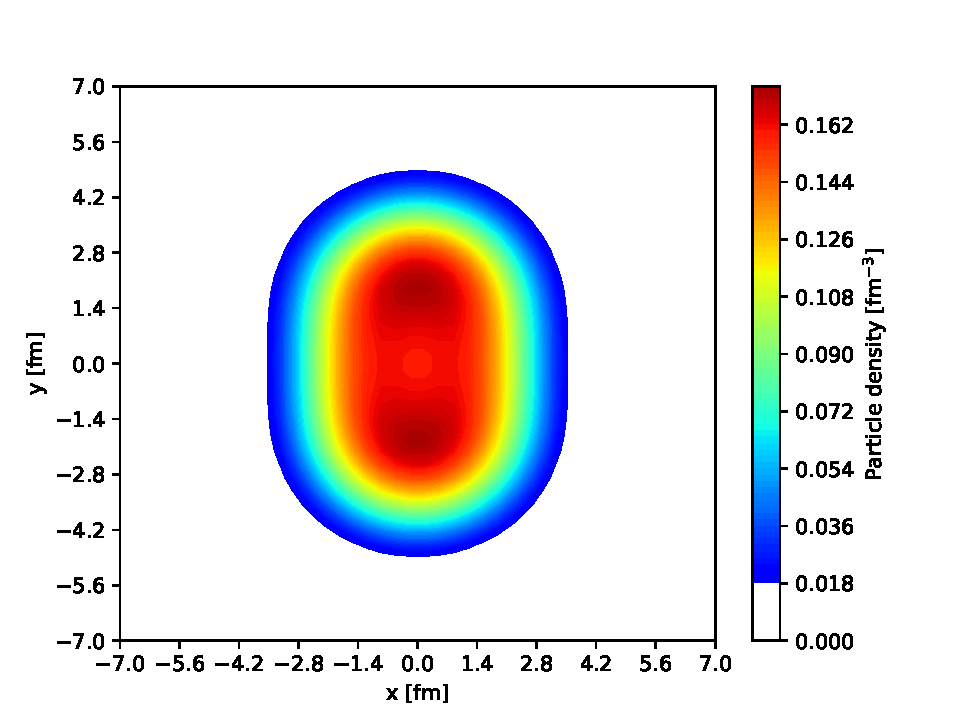
\includegraphics[width=1.0\linewidth]{Images/mg_gs_density_axial.pdf}
  \caption{Magnesium ground state density, calculation done on a box $[-10, 10]$ fm, step size 0.33 fm, SKM* parametrization}
  \label{fig:mg_gs_density_axial}
\end{figure}
\subsubsection{Deformation curve}
In figure \ref{fig:mg_no_pair_deformation}, a deformation curve is shown for $^{24}$Mg, without pairing. It shows the same minimum as the unconstrained calculation at $\beta_2=0.399$. To counteract the sharp rise in CPU time, due to the high number of points in the curve, a coarser grid is used, hence the different energy value than the one reported in table \ref{tab:mg_table}.
\begin{figure}[h]
  \centering
  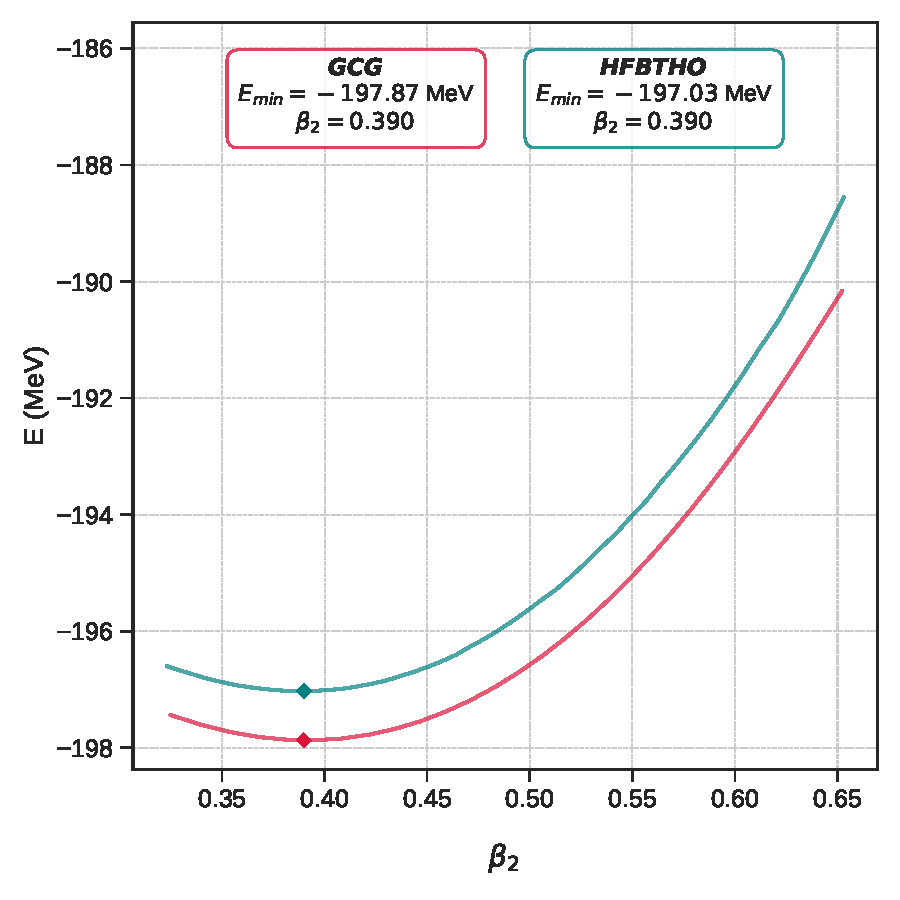
\includegraphics[width=0.8\linewidth]{Images/mg_nopair_curve.pdf}
  \caption{Magnesium deformation curve, no pairing interaction, calculation done on a box $[-10, 10]$ fm, step size 0.66 fm, SKM* parametrization.}
  \label{fig:mg_no_pair_deformation}
\end{figure}